\documentclass[a4paper]{article}
\usepackage{beamerarticle}

% \documentclass[aspectratio=169, ignorenonframetext]{beamer}
\usepackage{pgf}
%
\mode<article>{\usepackage{fullpage}}
\mode<presentation>
{
%   \usetheme{Madrid}
%   \useinnertheme{circles}
  \setbeamertemplate{navigation symbols}{}
%   \usetheme[hideothersubsections, width=2.4cm]{Hannover}
%   \usetheme{Antibes}
  \usetheme{Montpellier}
%   \usecolortheme{seahorse}
%   \setbeamertemplate{footline}
%   {%
%     \begin{beamercolorbox}{section in head/foot}
%       \usebeamercolor{bg}
% %       \hskip 1em \footnotesize \insertframenumber{} / \inserttotalframenumber\hskip 41em 
\includegraphics[height = .5cm]{../../../../bilder/cc_by-nc_eu.png}
% % cc_by-nc_eu.png: 403x141 px, 72dpi, 14.22x4.97 cm, bb=0 0 403 141
%
% % bwslogo_3.png: 476x392 px, 300dpi, 4.03x3.32 cm, bb=0 0 114 94
%
%       %\hskip 5em
%       %       \input{../bilder/cc_by.png}
%       %\includegraphics[height=.5cm]{../../../../bilder/bwslogo_3.png}
%     \end{beamercolorbox}%
%   }
  \usepackage{beamerfoils}
}

\usepackage[german]{babel}
\usepackage[utf8]{inputenc}
\usepackage{times}
\usepackage[T1]{fontenc}
\usepackage{eurosym}
\usepackage{graphicx}
\usepackage{amsmath}
\usepackage[siunitx,european]{circuitikz}
\usepackage{ulem}
\usepackage{listings}
%
\lstset{numbers=left, numberstyle=\tiny, stepnumber=2, numbersep=5pt, language = C++, alsolanguage=XML}
% \MyLogo{\includegraphics[height=1cm]{../../../../bilder/bwslogo_3.png}}
% % \includegraphics{../../bilder/bwslogo_3.png}
% % bwslogo_3.png: 476x392 px, 300dpi, 4.03x3.32 cm, bb=
%
\only<article>{
\usepackage[colorlinks=true,linkcolor=blue,filecolor=magenta,urlcolor=cyan]{hyperref}
}

\only<presentation>{
  \usepackage{hyperref}
}


\title{Arbeitsunterlagen zu FOS ET (12.1 und 12.6)}
\date{V 0.1 - im Aufbau\\ Stand: \today}%\\

\institute[BWS Hofheim]{Brühlwiesenschule, Hofheim}
\author{Thomas Maul}

\titlegraphic{Für eigene Teile gilt: 
\includegraphics[height=1cm]{cc_by-nc_eu.png}}

\begin{document}
\only<article>{
\maketitle
\tableofcontents
\clearpage
}
\begin{frame}<beamer>
  \titlepage
  % \hyperlink{Teil_2}{\beamerbutton{Go part 2}}
\end{frame}


\part{Themenfeld 12.1 - Gleichstromnetzanalyse}
\begin{frame}
  \partpage
  \tableofcontents[hidesubsections]
\end{frame}

\section{Zweipole}
In der Elektrotechnik werden Bauteile, die zwei Abschlüsse haben als Zweipole bezeichnet. Dies können jeweils einzelne Widerstände, Spulen und Kondensatoren sein. Manchmal ist es praktisch eine (Teil-)Schaltung als einen Zweipol darzustellen und in Berechnungen als ein virtuelles Bauteil zu verwenden.
\begin{frame}{Zweipole}
  In der Schaltung unten sollen die Widerstände $R_3$ bis $R_5$ als ein virtuelles Bauteil dargestellt werden.
  \begin{figure}[htb]
    \begin{circuitikz}
      \draw (0,0) to[vsource, l=$U_{q1}$] (0,2);
      \draw (0,2) to[R=$R_1$] (2,2) node[circ]{} node[above]{A} to[R=$R_2$] (2,0) node[circ]{} node[below]{B}  -- (0,0);
      \draw (2,2) -- (3,2) node[ocirc]{} node[above]{C} -- (4,2) to[R=$R_3$]
      (4,0) -- (3,0) node[ocirc]{} node[below]{D} -- (2,0);
      \draw (4,2) to[R=$R_4$] (6,2);
      \draw (6,2) to[R=$R_5$] (6,0) --
      %(6,2) to[vsource, l=$U_2$] (6,0) --
      (6,0) -- (4,0);
    \end{circuitikz}
%       \caption{Schaltung 1}
    \label{fig:InfoZweipole1}
  \end{figure}
\end{frame}
Es soll so aussehen, als ob nur ein Widerstand rechts von den Punkten C und D wäre. Durch Reihenschaltung von $R_4$ und $R_5$ zu $R_{45}$ und anschließender Parallelschaltung mit $R_3$ kann ich dies erreichen (siehe Bild \ref{fig:BerechnungErsatzR}). Der Widerstand $R_{3||45}$ verhält sich für die Schaltung wie die Widerstände $R_3$, $R_4$ und $R_5$.

Ich lege für die Widerstände folgende Werte fest:\\

\begin{frame}{Werte für Berechnung}
  \begin{columns}[t]
    \begin{column}{2cm}
      $R_1 = 10 \Omega$\\ $R_2 = 20 \Omega$\\ $ R_3 = 30 \Omega$\\ $ R_4 = 40 \Omega$\\ $ R_5 = 50 \Omega$\\ $U_{q1} = 5V,$ \\
        $U_{q2} = 12V$
      \label{comp:WiderstaendeSchaltung1}
    \end{column}
    \begin{column}{7cm}
      \begin{figure}[htb]
        \begin{circuitikz}
          \draw (0,0) to[vsource, l=$U_{q1}$] (0,2);
          \draw (0,2) to[R=$R_1$] (2,2) node[circ]{} node[above]{A} to[R=$R_2$] (2,0) node[circ]{} node[below]{B}  -- (0,0);
          \draw (2,2) -- (3,2) node[ocirc]{} node[above]{C} -- (4,2) to[R=$R_3$]
          (4,0) -- (3,0) node[ocirc]{} node[below]{D} -- (2,0);
          \draw (4,2) to[R=$R_4$] (6,2);
          \draw (6,2) to[R=$R_5$] (6,0) --
          %(6,2) to[vsource, l=$U_2$] (6,0) --
          (6,0) -- (4,0);
        \end{circuitikz}
%         \caption{Schaltung 1}
        \label{fig:InfoZweipole2}
      \end{figure}
    \end{column}
  \end{columns}
%       Jetzt kann ich den Gesamtwiderstand $R_{3||45}$ berechnen.
\end{frame}
\begin{frame}{Berechnung des Ersatzwiderstands}
  \begin{columns}[t]
    \begin{column}{4cm}
\begin{align}
  R_{45} &= R4 + R5\\
  R_{45} &= 40 \Omega + 50 \Omega \\
  R_{45} &= 90 \Omega\\
% \end{align}
% \begin{align}
  \frac{1}{R_{3||45}} &= \frac{1}{R_3} + \frac{1}{R_45}\\
  \frac{1}{R_{3||45}} &= \frac{1}{30\Omega} + \frac{1}{90\Omega}\\
  R_{3||45} &= 22,5\Omega
  \label{eq:zweipolr345}
\end{align}
    \end{column}
    \begin{column}{4cm}
      \begin{figure}[htb]
    \begin{circuitikz}
      \draw (0,0) to[vsource, l=$U_{q1}$] (0,2);
      \draw (0,2) to[R=$R_1$] (2,2) node[circ]{} node[above]{A} to[R=$R_2$] (2,0) node[circ]{} node[below]{B}  -- (0,0);
      \draw (2,2) -- (3,2) node[ocirc]{} node[above]{C} -- (3.5,2) to[R=$R_{3||45}$]
      (3.5,0) -- (3,0) node[ocirc]{} node[below]{D} -- (2,0);
    \end{circuitikz}
    \caption{Berechnung des Erstatwiderstands}
    \label{fig:BerechnungErsatzR}
  \end{figure}
    \end{column}
  \end{columns}
\end{frame}
Jetzt kann ich den Gesamtwiderstand $R_{3||45}$ berechnen. Ich kann jedoch nicht mehr einzelne Spannungen oder Ströme messen oder darstellen.

Der virtuelle Widerstand $R_{3||45}$ ersetzt die Schaltung der drei Widerstände. Das Gleiche ist mit allen passiven Bauteilen möglich. Auch aktive Bauteile (Quellen, Transistor, FET, \dots) kann man durch einen Zweipol ersetzen.

\begin{frame}{Übungen zu Zweipole I}
  Berechnen Sie jeweils den Ersatzwiderstand zwischen den Klemmen C und D zur Schaltung unten.
\begin{description}
 \item[a] $R1 = R2 = 220 \Omega \ R3 = R5 = 230 \Omega \ R4 = 470 \Omega$
 \item[b] $R1 = R2 = R3 = R5 = 230 \Omega \ R4 = 470 \Omega$
 \item[c] $R1 = R2 = R4 = R5 = 230 \Omega \ R3 = 470 \Omega$
\end{description}
      \begin{figure}[htb]
        \begin{circuitikz}
          \draw (0,0) to[vsource, l=$U_{q1}$] (0,2);
          \draw (0,2) to[R=$R_1$] (2,2) node[circ]{} node[above]{A} to[R=$R_2$] (2,0) node[circ]{} node[below]{B}  -- (0,0);
          \draw (2,2) -- (3,2) node[ocirc]{} node[above]{C} -- (3.5,2) to[R=$R_3$]
          (6,0) -- (3,0) node[ocirc]{} node[below]{D} -- (2,0);
          \draw (3.5,2) -- (4,2) to[R=$R_4$] (6,2);
          \draw (6,2) to[R=$R_5$] (6,0);
        \end{circuitikz}
        \caption{Schaltung zu Übung Ersatzzweipol - Teil 1}
      \end{figure}

    \label{fig:UebZweipole1}
\end{frame}

\begin{frame}{Übungen zu Zweipole II}
  Berechnen Sie jeweils den Ersatzwiderstand zwischen den Klemmen C und D zur Schaltung unten.
  \begin{description}
    \item[a] $R1 = R2 = 220 \Omega \ R3 = R5 = 230 \Omega \ R4 = 470 \Omega$
    \item[b] $R1 = R2 = R3 = R5 = 230 \Omega \ R4 = 470 \Omega$
    \item[c] $R1 = R2 = R4 = R5 = 230 \Omega \ R3 = 470 \Omega$
  \end{description}
  \begin{figure}[htb]
    \begin{circuitikz}
      \draw (0,0) to[vsource, l=$U_{q1}$] (0,2);
      \draw (0,2) to[R=$R_1$] (2,2) node[circ]{} node[above]{A} to[R=$R_2$] (2,0) node[circ]{} node[below]{B}  -- (0,0);
      \draw (2,2) -- (3,2) node[ocirc]{} node[above]{C} -- (3,2);
      \draw (5,2) to[R=$R_3$] (3,0) node[ocirc]{} node[below]{D} -- (2,0);
      \draw (3,2) to[R=$R_4$] (5,2);
      \draw (5,2) to[R=$R_5$] (5,0);
      \draw (5,0) -- (3,0);
    \end{circuitikz}
    \caption{Schaltung zu Übung Ersatzzweipol - Teil 2}
  \end{figure}

  \label{fig:UebZweipole2}
\end{frame}



\section{Überlagerungssatz}
\begin{frame}<beamer>
  \frametitle{Inhalt}
  \tableofcontents[currentsection, hideothersubsections]
\end{frame}

Wenn in einer Schaltung, man spricht auch von elektrischen Netzwerken, mehr als eine Quelle vorhanden ist, speisen alle Quellen gemeinsam die Schaltung mit Energie. Um in der Schaltung unten (Abbildung \ref{fig:SchaltungZweiQuellenAktiv}) zu berechnen, wie viel Strom durch den Widerstand $R_2$ fließt muss ich wissen, wie viel Strom die Quelle $U_1$ und wie viel die Quelle $U_2$ an den Widerstand abgibt.
\begin{frame}{Zwei Spannungsquellen U1 und U2}
  \begin{figure}[htb]
    \begin{circuitikz}
      \draw (0,0) to [vsource, l=$U_{q1}$] (0,4);
      \draw (0,4) to [R=$R_1$] (2,4) node[circ]{} node[above]{A} to [short, i>_=$I_2$] (2,3);
      \draw (2,3) to [R=$R_2$,  v=$U_2$] (2,0) node[circ]{} node[below]{B}  -- (0,0);
      \draw (2,4) -- (3,4) to[short, -*] (4,4) to[short] (4,3)  to[R=$R_3$]
      (4,0) -- (3,0) -- (2,0);
      \draw (4,4) to [R=$R_4$] (6,4);
      \draw (6,4) to [R=$R_5$] (6,2);
      \draw (6,2) to [vsource, l=$U_{q2}$] (6,0) -- (6,0);
      \draw (6,0) to [short, -*] (4,0);
    \end{circuitikz}
    \caption{Zwei Quellen aktiv}
    \label{fig:SchaltungZweiQuellenAktiv}
  \end{figure}
  $R1 = 10\Omega ,\ R2 = 20 \Omega ,\ R3 = 30\Omega ,\ R4 = 40 \Omega ,\ R5 = 50 \Omega$

\end{frame}

Mit einem Messgerät kann ich die Spannung an $R_2$ messen, den Strom, der durch $R_2$ fließt ebenfalls. Rechnerisch muss ich die Schaltung so verändern, dass jeweils nur die eine Quelle aktiv ist. Die anderen Spannungsquellen werden kurzgeschlossen. Wenn Stromquellen in der Schaltung sind werden diese aufgetrennt. Innenwiderstände der Quellen (hier $R_1$ zu $U_1$ und $R_5$ zu $U_2$ bleiben dabei in der Schaltung. Die Teilspannung an $R_2$, die ich jetzt errechnen kann, nenne ich $U_{2'}$.
\subsection{Nur Quelle U1 aktiv}
  \begin{frame}{Nur Quelle U1 aktiv}
  \begin{figure}[htb]
    \begin{circuitikz}
      \draw (0,0) to[vsource, l=$U_{q1}$] (0,4);
      \draw (0,4) to[R=$R_1$] (2,4) node[circ]{} node[above]{A} to [short, i>_=$I_2$] (2,3);
      \draw (2,3) to [R=$R_2$,  v=$U_{2}$] (2,0) node[circ]{} node[below]{B}  -- (0,0);
      \draw (2,4) -- (3,4) to[short, -*] (4,4) to[short] (4,3)  to[R=$R_3$]
      (4,0) -- (3,0) -- (2,0);
      \draw (4,4) to[R=$R_4$] (6,4);
      \draw (6,4) to[R=$R_5$] node[ocirc]{} (6,2) --
       node[ocirc]{} (6,0) --
      (6,0) to[short, -*] (4,0);
    \end{circuitikz}
    \caption{Nur Quelle 1 aktiv}
    \label{fig:Schaltung4_1}
  \end{figure}
  $R1 = 10\Omega ,\ R2 = 20 \Omega ,\ R3 = 30\Omega ,\ R4 = 40 \Omega ,\ R5 = 50 \Omega$
\end{frame}

$R_2$ wird jetzt mit dem Ersatzwiderstand $R_{3||45}$ parallel geschaltet.
\begin{frame}{Berechnung Ersatzwiderstand I}
\begin{align}
  U_{2'} &= I_2 * R_2||R_3||R_4+R_5\\
  U_{2'} &= I_2 *\frac{1}{\frac{1}{R_2}+\frac{1}{R_3}+\frac{1}{R_4+R_5}}
\end{align}
$I_2$ ist nicht bekannt.
\end{frame}
Zur Berechnung müssten jedoch entweder $I_2$ oder $U_2$ bekannt sein. Somit hilft diese Formel noch nicht endgültig. Bekannt sind die Widerstandswerte und die Spannung $U_1$. Mit der Formel eines Spannungsteilers kann ich die Spannung an der Parallelschaltung ausrechnen ohne $I_2$ zu kennen.
\begin{frame}{Berechnung Ersatzwiderstand II}
\begin{align}
U_{q1} &= U_1 + U_2\\
U_2 &= U_{q1}*\frac{R_2||R3||R45}{R!+ R_2||R3||R45}
\end{align}
\end{frame}
In der Festlegung \ref{comp:WiderstaendeSchaltung1} (Seite \pageref{comp:WiderstaendeSchaltung1}) habe ich die Werte für die Widerstände und die Spannungen der Quellen festgelegt. In Formel (\ref{eq:zweipolr345}, Seite \pageref{eq:zweipolr345}) habe ich den Ersatzwiderstand für $R_{3||45}$ berechnet. Hier setze ich die Werte in die Formeln ein:
\begin{frame}{Einsetzen I}
  \begin{align}
U_{2'} &= U_{q1}*\frac{R_2||R3||R45}{R1 + R_2||R3||R45}\\
U_{2'} &= U_{q1}*\frac{\frac{1}{\frac{1}{R_2}+\frac{1}{R_3}+\frac{1}{R_4+R_5}}}{R_1 + \frac{1}{\frac{1}{R_2}+\frac{1}{R_3}+\frac{1}{R_4+R_5}}}\\
  \end{align}
\end{frame}
\begin{frame}{Einsetzen II}
  \begin{align*}
    U_{2'} &= U_{q1}*\frac{R_2||R3||R45}{R1 + R_2||R3||R45}\\
    U_{2'} &= U_{q1}*\frac{\frac{1}{\frac{1}{R_2}+\frac{1}{R_3}+\frac{1}{R_4+R_5}}}{R_1 + \frac{1}{\frac{1}{R_2}+\frac{1}{R_3}+\frac{1}{R_4+R_5}}}\\
  \end{align*}
  \begin{align}
    U_{2'} &= 5V*\frac{22,5\Omega}{10\Omega + 22,5\Omega}\\
  U_{2'} &= 5V * 0,69\\
  U_{2'} &= 3,46V
  \end{align}
\end{frame}

\subsection{Nur Quelle U2 aktiv}
\begin{frame}{Nur Quelle U2 aktiv}
\begin{figure}[htb]
  \begin{circuitikz}
    \draw (0,0) to node[ocirc]{} (0,2) to node[ocirc]{} (0,3) -- (0,4) ;
    \draw (0,4) to [R=$R_1$] (2,4) node[circ]{} node[above]{A} to [short, i>_=$I_2$] (2,3);
    \draw (2,3) to [R=$R_2$,  v=$U_2$] (2,0) node[circ]{} node[below]{B}  -- (0,0);
    \draw (2,4) -- (3,4) to[short, -*] (4,4) to[short] (4,3)  to[R=$R_3$]
    (4,0) -- (3,0) -- (2,0);
    \draw (4,4) to [R=$R_4$] (6,4);
    \draw (6,4) to [R=$R_5$] (6,2);
    \draw (6,2) to [vsource, l=$U_{q2}$] (6,0) -- (6,0);
    \draw (6,0) to (4,0);
  \end{circuitikz}
  \caption{Nur Quelle zwei aktiv}
  \label{fig:Schaltung4_2}
\end{figure}
$R1 = 10\Omega ,\ R2 = 20 \Omega ,\ R3 = 30\Omega ,\ R4 = 40 \Omega ,\ R5 = 50 \Omega$
\end{frame}
In diesem Fall ist $R_2$ parallelgeschaltet mit $R_1$ und $R_3$.
\begin{frame}{Quelle 2, Einsetzen I}
  \begin{align}
    U_{2''} &= U_{q2}*\frac{\frac{1}{\frac{1}{R_1}+\frac{1}{R_2}+\frac{1}{R_3}}}{R_4 + R_5 + \frac{1}{\frac{1}{R_1}+\frac{1}{R_2}+\frac{1}{R_3}}}\\
    \end{align}
\end{frame}

\begin{frame}{Quelle 2, Einsetzen II}
  \begin{align}
    U_{2''} &= U_{q2}*\frac{\frac{1}{\frac{1}{R_1}+\frac{1}{R_2}+\frac{1}{R_3}}}{R_4 + R_5 + \frac{1}{\frac{1}{R_1}+\frac{1}{R_2}+\frac{1}{R_3}}}\\
    U_{2''} &= 12\,V*\frac{\frac{1}{\frac{1}{10\Omega}+\frac{1}{20\Omega}+\frac{1}{30\Omega}}}{40\Omega + 50\Omega + \frac{1}{\frac{1}{10\Omega}+\frac{1}{20\Omega}+\frac{1}{30\Omega}}}\\
    U_{2''} &= 0,24V
  \end{align}
\end{frame}

\begin{frame}{Addition}
Zum Abschluss werden die beiden Teilspannungen addiert.
  \begin{align}
    U_2 &= U_{2'} + U_{2''}\\
    U_2 &= 3,46V + 0,24V\\
    U_2 &= 3,7V
  \end{align}
\end{frame}



%   \section{Maschenstromanalyse}
%
%
%   $\begin{vmatrix}
%     1 & 0 & 0 \\
%     0 & 1 & 0 \\
%     0 & 0 & 1 \\
%   \end{vmatrix}$
%   \\
%   $\begin{array}{|rr|r|}
%     1 & 0 & 0 \\
%     0 & 1 & 0 \\
%     0 & 0 & 1 \\
%   \end{array}$
%   \section{Knotenpotentialanalyse}

\part{Themenfeld 12.6 - Elektrisches und magnetisches Feld}
\begin{frame}
\partpage
\end{frame}
\section{Ladungen, Kräfte}
\only<presentation>{
\begin{frame}{Elektronen und Atome}
  \begin{itemize}
    \item Die Materie besteht aus Atomen.
    \item Kern: Protonen und Neutronen, Hülle: Elektronen
    \item Bei Leitern: Elektronen \glq mobil\grq, bei Nichtleitern fest(er)
    \item Reibung von 2 Nichtleitern (Stoff und Glasstab)$\Rightarrow$ Ladungstrennung
  \end{itemize}
\end{frame}
}
Die Materie besteht aus Atomen. Diese wiederum aus einem Kern mit Protonen und Neutronen und einer Hülle aus Elektronen. Bei einigen Atomen, zum Beispiel Metalle sind, ist es leicht möglich einzelne Elektronen aus der Hülle zu entfernen. Dies führt zur elektrischen Leitung - dem elektrischen Strom.

Bei Stoffen, die nicht leitend sind, lassen sich die Elektronen nicht oder nur schwer aus der Hülle entfernen.

Wenn man zwei nicht leitende Gegenstände, zum Beispiel einen Glasstab und ein Stück Stoff aneinander reibt, werden durch die Reibung Elektronen in einem der beiden Gegenstände aus der Hülle herausgerissen und in die Atomhüllen der Atome des anderen Gegenstands übertragen. In diesem Moment spricht man davon, dass beide Gegenstände elektrisch geladen sind.
\begin{frame}{Katze mit Styroporflocken}
\begin{figure}[htb]
  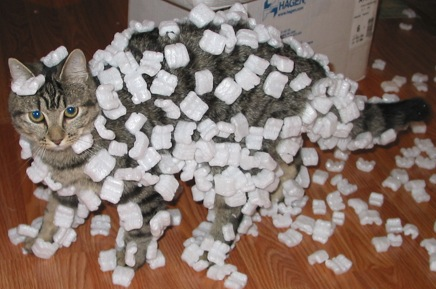
\includegraphics{Cat_demonstrating_static_cling_with_styrofoam_peanuts.jpeg}
%    Cat_demonstrating_static_cling_with_styrofoam_peanuts.jpeg: 436x289 px, 180dpi, 6.15x4.08 cm, bb=
  \caption{Katze mit Styroporflocken}
  \label{abb:CatWidthStyropor}
  \footnote{Quelle: Von Original image: Sean McGrath from Saint John, NB, CanadaDerived image: Black Rainbow 999 - Diese Datei ist ein Ausschnitt aus einer anderen Datei, CC BY 2.0, https://commons.wikimedia.org/w/index.php?curid=60287175}
\end{figure}
\end{frame}

\only<presentation>{
  \begin{frame}{Anziehung und Abstoßung von Ladungen}
      \begin{itemize}
        \item gleichnamige Ladungen stoßen sich ab.
        \item ungleichnamige Ladungen ziehen sich an.
        \item bei Elektrostatik gibt es keine Bewegung, nur Kräfte
      \end{itemize}
  \end{frame}
}

Elektrische Ladungen, die gleich sind (zwei positive Ladungen oder zwei negative) stoßen sich ab. Ladungen, die unterschiedlich sind, ziehen sich an.

Die Abstoßung und Anziehung kann man als Kräfte berechnen und in gewissen Grenzen messen.

Wenn sich die Ladungen nicht zwischen den Körpern bewegen und auch nicht innerhalb des Körpers, nennt man dies einen statischen Zustand. Die Ladung ist vorhanden, die Kräfte sind vorhanden aber es gibt keine Bewegung. Unter idealen Bedingungen bleibt der Zustand dauerhaft bestehen. In der Schule vereinfachen wir. Eine Ladung ist als punktförmig definiert, sie hat keine Ausdehnung, für die Elektrostatik gilt, dass sie ohne äußere Einflüsse unverändert bleibt. Elektronen und Ladungen bewegen sich nicht.

\section{Energieerhaltung und Einheit}
Unabhängig von den Vereinfachungen gilt, dass es einen Energieerhaltungssatz gibt. Energie kann nur umgewandelt werden. Potentielle in kinetische oder chemische Energie. Energie kann innerhalb eines geschlossenen Systems (wir gehen davon aus, dass unsere System alle geschlossen sind) nicht entstehen und nicht vernichtet werden. Damit bleibt die Gesamtladung auch immer identisch.

Die Elektrische Ladung wird in Coulomb (Einheit C) gemessen, $1 C = 1 As$. \\ Die Elementarladung (kleinste Einheit) beträgt: $e = 1,602 * 10^{-19} C$

Wenn eine positive Ladung und eine negative Ladung nahe beieinander existieren, bilden sich zwischen ihnen Kräfte. Zusätzlich kann man ein elektrostatisches Feld messen. Das Feld wird als Linien dargestellt. Die Feldlinien beginnen bei der positiven Ladung und enden an der negativen Ladung.

\section{Abmaße von Ladungen}
Eine Punktladung wird als unendlich kleiner Punkt definiert. Wichtig ist, dass der Durchmesser der Ladung wesentlich kleiner ist, als der Abstand zu einer anderen Ladung.

Eine Linienladung stellt eine Linie dar, auf der sich die (gleichnamigen) Ladungen befinden. Die Linie ist relativ gesehen dünn, es kann zum Beispiel ein Draht sein, der im Raum als Linie dargestellt werden kann. Die Ladungen sind gleichmäßig auf der kompletten Strecke verteilt.

Eine Flächenladung verteilt sich auf einer Fläche gleichmäßig. In der Regel passiert dies bei metallischen Flächen oder anderen Flächen, die gut leitend sind. Hier verteilen sich die Ladungen auf der gesamten Fläche gleichmäßig.

Eine Raumladung stellt eine gleichmäßige Verteilung elektrischer Ladungen innerhalb eines Volumens dar.

\section{Vektoren}
Ein Vektor beschreibt den Abstand und die Richtung zwischen zwei Punkten. In Bild \ref{fig:ZweiVektoren} sind zwei Vektoren: $\vec{v}_1= \left(\begin{array}{c} 1 \\ 2 \end{array}\right)$ und  $\vec{v}_2= \left(\begin{array}{c} 2 \\ 1 \end{array}\right)$. Jeder Vektor beschreibt einen Punkt im Koordinatensystem. Der Startpunkt des Vektors muss nicht im Punkt $\left(\begin{array}{c}0\\0\end{array}\right)$ sein. Daher beschreibt der Vektor eine Verschiebung eines Punkts um die Koordinaten (hier x und y).

Die Länge des Vektors, der sogenannte Betrag, wird mit der $\sqrt{\Delta x^2 + \Delta y^2}$ berechnet. Hier: \[|v_1| = \sqrt{(1 - 0) + (2 - 0)} = \sqrt{3}\].
\begin{frame}{Vektoren}
  \begin{figure}[htb]
    \begin{tikzpicture}
      \draw (-2,0) -- (2,0);
      \draw (0,-2) -- (0,2);
      %\draw node[circ] at (0,0){};
      \draw[->] (0,0) -- (1,2);
      \draw[->] (0,0) -- (2,1);
      \draw node at (0.8,1) {$\vec{v}_1$};
      \draw node at (1.4,0.4) {$\vec{v}_2$};
    \end{tikzpicture}

      $\vec{v}_1= \left(\begin{array}{c} 1 \\ 2 \end{array}\right)$ und  $\vec{v}_2= \left(\begin{array}{c} 2 \\ 1 \end{array}\right)$
    \caption{Zwei Vektoren in zweidimensionalen Raum}
    \label{fig:ZweiVektoren}
  \end{figure}
\end{frame}

Vektoren können addiert werden, dabei werden jeweils die X-Komponenten, Y-Komponenten und ggf. weitere Komponenten einzeln addiert.
\begin{align}
 \vec{v}_3 &= \vec{v}_1 + \vec{v}_2\\
 \vec{v}_3 &= \left(\begin{array}{c} 1 \\ 2 \end{array}\right) + \left(\begin{array}{c} 2 \\ 1 \end{array}\right)\\
 \vec{v}_3 &= \left(\begin{array}{c} 3 \\ 3 \end{array}\right)
\end{align}

\begin{frame}{Addition von Vektoren}
  \begin{figure}[htb]
    \begin{tikzpicture}
      \draw (-2,0) -- (2,0);
      \draw (0,-2) -- (0,2);
      %\draw node[circ] at (0,0){};
      \draw[->] (0,0) -- (1,2);
      \draw[->] (0,0) -- (2,1);
      \draw[->] (1,2) -- (3,3);
      \draw[->] (0,0) -- (3,3);
      \draw node at (0.9,1.2) {$\vec{v}_1$};
      \draw node at (1.4,0.4) {$\vec{v}_2$};
      \draw node at (1.6,2) {$\vec{v'}_2$};
      \draw node at (2,1.5) {$\vec{v}_3$};
    \end{tikzpicture}

    $\vec{v}_1= \left(\begin{array}{c} 1 \\ 2 \end{array}\right)$, $\vec{v}_2= \left(\begin{array}{c} 2 \\ 1 \end{array}\right)$, $\vec{v'}_2 = \vec{v}_2$  und $\vec{v}_3= \left(\begin{array}{c} 3 \\ 3 \end{array}\right)$
    \caption{Zwei Vektoren in zweidimensionalen Raum}
    \label{fig:ZweiVektorenAddiert}
  \end{figure}
\end{frame}





\section{Literatur}
\begin{frame}{Literatur}
\begin{description}
  \item[Wikibooks] https://de.wikibooks.org/wiki/Elektrostatik
  \item[Marinescu, Marlene]  Elektrische und magnetische Felder,
  Eine praxisorientierte Einführung; A 3 (2012); Springer
\end{description}
\end{frame}

  \listoffigures
%   \listoftables


  \label{LastPage}
\end{document}
